\documentclass[12pt,a4paper]{article}%
\usepackage{CJKutf8}
\usepackage{makeidx}
\makeindex
\usepackage{bm}
\usepackage{framed} % Easier way to use Framebox
\usepackage{pdfpages} % Import PDF in latex document
\usepackage{listings}
\usepackage{slashbox}
\usepackage{array}
\usepackage{enumitem}
\usepackage{amsmath, amssymb, amsthm}  % For mathematical symbols
\usepackage{colortbl,color}
\usepackage{xcolor}
\usepackage{auto-pst-pdf}
\usepackage{graphicx,psfrag}
\usepackage{tabularx,array}
\usepackage{booktabs}
\usepackage{multirow}
\usepackage{multicol}
\usepackage[subfigure]{tocloft}
\usepackage[tight]{subfigure}
\usepackage{float,booktabs,threeparttable}
\usepackage{caption}


\usepackage{longtable}
\usepackage{appendix}

\usepackage{pdfpages}
\usepackage{blkarray} %For adding Matrix label on row and column
\usepackage{url}
\usepackage{indentfirst} % indent the first paragraph of new section
\usepackage{titlesec} % change the way \subsubsubsection formats

\def\se{{\rm se}}
%\newcommand{\red}{\color{red}}
\linespread{1.5}  % The linespread is 1.5.

% Numbered theorems, definitions, algorithm and lemmas ======================================================================
\newtheorem{thm}{Theorem}  % Define new theorem.
\newtheorem{alg}{Algorithm}[section]  % Define new algorithm.
\newtheorem{definition}{Definition}
% ===========================================================================================================================

% For writing pseudo code ======================================================================
\usepackage{algorithm}% http://ctan.org/pkg/algorithms
\usepackage{algpseudocode}% http://ctan.org/pkg/algorithmicx
% ===========================================================================================================================

\theoremstyle{definition}
\theoremstyle{plain}
\setcounter{secnumdepth}{5}


\renewcommand{\contentsname}{Table of Contents}
\renewcommand{\listfigurename}{List of Figures}
\renewcommand{\listtablename}{List of Tables}
\renewcommand{\figurename}{\footnotesize Figure}
\renewcommand{\tablename}{\footnotesize Table}
\newcommand{\loflabel}{Figure}
\newcommand{\lotlabel}{Table}
\setlength{\abovecaptionskip}{0pt}


\renewcommand{\cftsecnumwidth}{7em}
\renewcommand{\appendixpagename}{\Large Appendix} % \ctxfb
\renewcommand{\arraystretch}{1.2}

\usepackage{appendix}



%%%%%%%%%%%%

\newtheorem{lma}{\textbf{Lemma}}

% ======================== Set length ========================
\setlength{\columnsep}{1cm}
\setlength\parindent{0pt}
\textheight = 22cm
\textwidth = 16.5cm
\hoffset=-1cm
\footskip=40pt
\renewcommand*{\arraystretch}{0.8}
% ============================================================
% ======================== Paragraph Indent ========================
\setlength{\parindent}{1em}
\setlength{\parskip}{1em}
% ==================================================================
% =============================
% Equation numbering
\numberwithin{equation}{section}
% =============================
% ======================== SubSubSubSection Format ========================
\titleclass{\subsubsubsection}{straight}[\subsection]

\newcounter{subsubsubsection}[subsubsection]
\renewcommand\thesubsubsubsection{\thesubsubsection.\arabic{subsubsubsection}}

\titleformat{\subsubsubsection}
  {\normalfont\normalsize\bfseries}{\thesubsubsubsection}{1em}{}
\titlespacing*{\subsubsubsection}
{0pt}{3.25ex plus 1ex minus .2ex}{1.5ex plus .2ex}
% ==================================================================



\begin{document}

\setcounter{section}{3}
\section{Classifications}
\subsection{\textbf{Logistic Regression}}
\subsubsection{\textbf{Logistic Model}}

Logistic function:
\begin{gather}
p(x_{i}) = \frac{e^{\beta^{T}x_{i}}}{1+e^{\beta^{T}x_{i}}} = \frac{1}{1+e^{-\beta^{T}x_{i}}},~~ 0 \leq p(x_{i}) \leq 1, ~~ -\infty < x_{i} < \infty
\label{logistic-model}
\end{gather}

The logistic function will always produce an S-shaped curve.
\begin{figure}[H]
\centering
\psfrag{A}[c][l]{$X$}
\psfrag{B}[c][l]{$p(X)$}
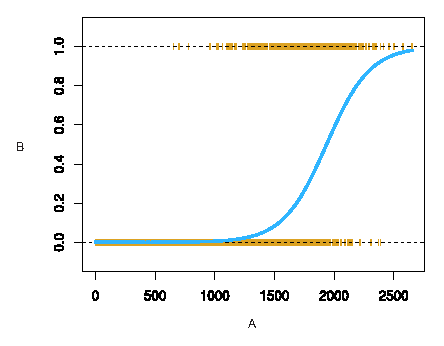
\includegraphics[scale=1]{images//4_2.eps}
\\~\\
\caption{}\label{figure-4.2}
\end{figure}

With a bit of manipulation, we will get a odds function:
\begin{gather}
\frac{p(x_{i})}{1-p(x_{i})} = e^{\beta^{T}x_{i}},~~ 0< \frac{p(x_{i})}{1-p(x_{i})} < \infty
\label{odds-function}
\end{gather}

The notation $p(x)$ can be interpreted as ${\rm Pr(Y=1|X=x)}$, which means the probability of $Y$ is True given $x$.
The equation \eqref{odds-function} imply the ratio of success compare to fail. For example, average nine of ten people go to school.
That means 9 times of people go to school compare to those who don't. So:
\begin{gather*}
p(x) = {\rm Pr(y=1|x)} = 9/10 \\
\frac{p(x)}{1-p(x)} = \frac{9/10}{1-9/10} = 9
\end{gather*}

By taking the logarithm of the odds function, we get
\begin{gather}
\log \bigg( \frac{p(x)}{1-p(x)} \bigg)= \beta^{T}x_{i}
\end{gather}

The left-hand side is called the log-odds or logit. We see that the logistic regression model has a logit that is linear in $X$.


\subsubsection{\textbf{Estimating the Regression Coefficients}}
To fit logistic model \eqref{logistic-model}, we use Maximum Likelihood to estimate the coefficients:
\begin{framed}
\begin{CJK}{UTF8}{cwmb}
\begin{definition}[Likelihood Function]
~\\
$X_{1},X_{2},\dots,X_{n}$ 為一組樣本大小為$n$之隨機樣本, 記為$X_{1},X_{2},\dots,X_{n} \stackrel{i.i.d.}{\sim} f_{X_{i}}(x_{i};\theta)$, 定義母體參數 $\theta$ 之 likelihood function:
\begin{gather*}
L(\theta) = f_{X_{1},X_{2},\dots,X_{n}}(x_{1},x_{2},\dots,x_{n}) = \prod_{i=1}^{n}f_{X_{i}}(x_{i};\theta)
\end{gather*}
可解讀為在不同的母體參數值$\theta$之下, 抽到這組觀測的隨機樣本($X_{1},X_{2},\dots,X_{n}$)之可能性
\end{definition}
\end{CJK}
\end{framed}

\subsubsubsection{\color{blue}{Maximum Likelihood Estimator, $\hat{\theta}_{\rm MLE}$}}
\begin{CJK}{UTF8}{cwmb}
找一個 $\theta$ 使得拿到這組隨機樣本($X_{1},X_{2},\dots,X_{n}$)的可能性為最大, 亦即, 找一個 $\theta$ 使得概似函數 $L(\theta)$ 為最大:
\begin{gather*}
\text{arg}\,\max\limits_{\theta}\,L(\theta), \text{求解}\,\hat{\theta}_{\rm MLE}
\end{gather*}
\end{CJK}

Unlike linear regression, we can no longer write down the MLE in closed form.
Instead, we need to use an optimization algorithm to compute it.
For this, we need to derive the gradient and Hessian. The likelihood function of logistic model:

\begin{gather}
L(\beta) = \prod_{i=1}^{n} p(x_{i};\beta)^{y_{i}} (1-p(x_{i};\beta))^{1-y_{i}},~\text{where~} R_{y_{i}}=\{0,1\}
\end{gather}

The log-likelihood of logistic model:
\begin{align*}
\ell(\beta)& = \sum\limits_{i=1}^{n} y_{i} \log p(x_{i};\beta)+(1-y_{i})\log (1-p(x_{i};\beta)) \\
		   & = \sum\limits_{i=1}^{n} y_{i} \log p(x_{i};\beta) + \log (1-p(x_{i};\beta)) - y_{i} \log (1-p(x_{i};\beta))\\
		   & = \sum\limits_{i=1}^{n} y_{i} \log \frac{p(x_{i};\beta)}{1-p(x_{i};\beta)} + \log (1-p(x_{i};\beta))  \\
		   & = \sum\limits_{i=1}^{n} y_{i}\beta^{T}x_{i}+ \log (\frac{1}{1+e^{\beta^{T}x_{i}}}) \\
 		   & = \sum\limits_{i=1}^{n} \{y_{i}\beta^{T}x_{i}-\log (1+e^{\beta^{T}x_{i}})\}
\end{align*}

First order partial differential of the log-likelihood function (gradient descent):
\begin{align*}
\frac{\partial \ell(\beta)}{\partial \beta} & = \sum\limits_{i=1}^{n} x_{i}(y_{i} - \frac{e^{\beta^{T}x_{i}}}{1+e^{\beta^{T}x_{i}}}) \\
 & = \sum\limits_{i=1}^{n} x_{i}(y_{i} - p(x_{i};\beta))
\end{align*}

Second order partial differential of the log-likelihood function (the s.o.c can transfer to a Hessian matrix):
\begin{align*}
\frac{\partial^{2} \ell(\beta)}{\partial \beta \partial \beta^{T}}
 & = \sum\limits_{i=1}^{n} x_{i}(-x_{i} \cdot \frac{e^{-\beta^{T} x_{i}}}{1+e^{-\beta^{T} x_{i}}} \cdot \frac{1}{1+e^{-\beta^{T} x_{i}}}) \\
 & = -\sum\limits_{i=1}^{n} x_{i}x_{i}^{T} p(x_{i};\beta) (1-p(x_{i};\beta))
\end{align*}

Starting with $\beta^{old}$, a single Newton update is
\begin{gather*}
\beta^{new} = \beta^{old} - \bigg(\frac{\partial^{2} \ell(\beta)}{\partial \beta \partial \beta^{T}}\bigg)^{-1} \frac{\partial \ell(\beta)}{\partial \beta}
\end{gather*}

Now we will try to simplify by vectorizing the model. Let $\mathbf{y}$ denote the vector of $y_{i}$,
$\mathbf{X}$ the $N \times (p+1)$ matrix of $x_{i}$ ($p$ predictors with one intercept),
$\mathbf{p}$ the vector of fitted probabilities with $i$th element $p(x_{i};\boldsymbol{\beta}^{\text{old}})$ and
$\mathbf{W}$ a $N \times N$ diagonal matrix of weights with $i$th diagonal element $p(x_{i};\boldsymbol{\beta}^{\text{old}})(1-p(x_{i};\boldsymbol{\beta}^{\text{old}}))$.
The structure of the notation and the model: ~\\~\\

$
\mathbf{y}_{N \times 1} = \begin{pmatrix}
  y_{1}  \\
  y_{2}  \\
  \vdots  \\
  y_{N}
 \end{pmatrix}
$,
$
\mathbf{X}_{N \times (p+1)} = \begin{pmatrix}
  1 & x_{11} & x_{12} & \cdots & x_{1p} \\
  1 & x_{21} & x_{22} & \cdots & x_{2p} \\
  \vdots & \vdots & \vdots & \ddots & \vdots  \\
  1 & x_{N1} & x_{N2} & \cdots & x_{Np}
 \end{pmatrix}
$, ~\\

$
\mathbf{p}_{N \times 1} = \begin{pmatrix}
  p(x_{1};\boldsymbol{\beta}^{\text{old}})  \\
  p(x_{2};\boldsymbol{\beta}^{\text{old}})  \\
  \vdots  \\
  p(x_{N};\boldsymbol{\beta}^{\text{old}})
 \end{pmatrix}
$,
$
\boldsymbol{\beta}^{\text{old}}_{(p+1) \times 1} = \begin{pmatrix}
  \beta_{0}  \\
  \beta_{1}  \\
  \beta_{2}  \\
  \vdots  \\
  \beta_{p}
 \end{pmatrix}
$,

\begin{gather*}
\footnotesize
\mathbf{W}_{N \times N} = \begin{pmatrix}
  p(x_{1};\boldsymbol{\beta}^{\text{old}})(1-p(x_{1};\boldsymbol{\beta}^{\text{old}})) & 0 & \cdots & 0 \\
  0 & p(x_{2};\boldsymbol{\beta}^{\text{old}})(1-p(x_{2};\boldsymbol{\beta}^{\text{old}})) & \cdots & 0 \\
  \vdots & \vdots & \ddots & \vdots  \\
  0 & 0 & \cdots & p(x_{N};\boldsymbol{\beta}^{\text{old}})(1-p(x_{N};\boldsymbol{\beta}^{\text{old}}))
 \end{pmatrix}
\end{gather*}

\begin{align*}
\frac{\partial \ell(\beta)}{\partial \beta} & = \mathbf{X}^{T}(\mathbf{y}-\mathbf{p}) \\
\frac{\partial^{2} \ell(\beta)}{\partial \beta \partial \beta^{T}}  & = -\mathbf{X}^{T} \mathbf{W} \mathbf{X} \\
\boldsymbol{\beta}^{\text{new}} &= \boldsymbol{\beta}^{\text{old}} + \big( \mathbf{X}^{T} \mathbf{W} \mathbf{X} \big)^{-1} \mathbf{X}^{T}(\mathbf{y}-\mathbf{p}) \\
 & = \big( \mathbf{X}^{T} \mathbf{W} \mathbf{X} \big)^{-1} \mathbf{X}^{T} \mathbf{W} \big( \mathbf{X} \boldsymbol{\beta}^{\text{old}} +  \mathbf{W}^{-1}(\mathbf{y}-\mathbf{p})\big) \\
 & = \big( \mathbf{X}^{T} \mathbf{W} \mathbf{X} \big)^{-1} \mathbf{X}^{T} \mathbf{W} \mathbf{z}
\end{align*}

Response of weighted least squares step, sometimes known as adjusted response:
\begin{gather}
\mathbf{z} = \mathbf{X} \boldsymbol{\beta}^{\text{old}} +  \mathbf{W}^{-1}(\mathbf{y}-\mathbf{p})
\end{gather}

The equations above solved repeatedly, since at each iteration $\mathbf{p}$ changes, and hence so does $\mathbf{W}$ and $\mathbf{z}$.
This algorithm is referred to as iteratively reweighed least squares (IRLS).

\begin{algorithm}[H]
\caption{Iteratively reweighted least squares (IRLS)}\label{euclid}
\begin{algorithmic}[1]
\State $\boldsymbol{\beta}^{\text{new}} =  \begin{pmatrix}  1 \\ \boldsymbol{\mathbf{\beta}}_{p}  \end{pmatrix} ;$
\Repeat
\State $\mathbf{p} = p(\mathbf{X};\boldsymbol{\beta}^{\text{new}})$
\State $\mathbf{W}_{N \times N} = \text{diag}(\mathbf{p} (1-\mathbf{p}))$
\State $\mathbf{z} = \mathbf{X}\boldsymbol{\beta}^{\text{new}}+ \mathbf{w}^{-1}(\mathbf{y}-\mathbf{p})$
\State $\boldsymbol{\beta}^{\text{new}} = (\mathbf{X}^{T} \mathbf{W} \mathbf{X})^{-1} \mathbf{X}^{T} \mathbf{W} \mathbf{z} $
\Until{calculate loss function to check converged;}
\end{algorithmic}
\end{algorithm}

\subsubsection{Discussion}
\begin{enumerate}
\item How to calculate the fitness of logistic model?
\item How to check the estimated coefficients is significant or not?
\item How to perform the hypothesis testing for logistic regression? 
\item What is the assumptions of logistic regression model?
\end{enumerate}

\subsection{\textbf{Linear Discriminant Analysis (LDA)}}

Difference between Linear Discriminant Analysis and Logistic Analysis:
\begin{itemize}
\item when the classes are well-separated, the parameter estimates for the logistic regression model are surprisingly unstable. LDA does not suffer from this problem
\item If $n$ is small and the distribution of the predictors $X$ is approximately normal in each of the classes, LDA is more stable than logistic regression
\item LDA is preferable when we have more than two response classes.
\item Logistic regression can take both qualitative and quantitative as predictor variables. However LDA can only take quantitative predictor variables, due to the assumption of multivariate Gaussian Distribution.
\item LDA assumes that the classes have a common covariance matrix
(Continuous random variable $X$)
\end{itemize}

\subsubsection{\textbf{Bayes Theorem for Classification}}
Classify an observation into one of $K$ classes, where $K \geq 2$.

Notations: 
\begin{itemize}
\item $Y$: The qualitative response variable with $K$ different categories, $R_{Y} = {1,\dots,K}$
\item $\pi_{k}$: The prior probability that a randomly chosen observation comes from the $k$th class
\item $f_{k}(X)$: The density function of $X$ for an observation comes form the $k$th class
\item $h^{*}(x)$: Indicate the class which the training data $x$ belongs to
\end{itemize}

\begin{framed}
Note:
\begin{gather*}
\hat{\pi}_{k} = n_{k}/n = \hat{Pr}(Y=k) \\
f_{k}(X) = Pr(X=x|Y=k)
\end{gather*}
\end{framed}
From the law of total probability, the above notations can be stated as below:
\begin{align*}
Pr(Y=k|X=x) &= \frac{P(X=x|Y=k)P(Y=k)}{\sum\limits_{\ell=1}^{K} P(X=x|Y=l)P(Y=l)} \\
  	        &= \frac{\pi_{k}f_{k}(x)}{\sum\limits_{\ell=1}^{K}\pi_{\ell}f_{\ell}(x)}
\label{lda}
\end{align*}
The abbreviation for $Pr(Y=k|X=x)$ will be denoted as $p_{k}(X)$ which is the posterior probability that an observation $X=x$ belongs to the $k$th class.
In the following section, we have to make assumptions and approximates $f_{k}(X)$ to build a classifier that approximates the Bayes classifier.

\begin{framed}
\begin{CJK}{UTF8}{cwmb}
\begin{definition}[The law of total probability]
~\\
設 $A_{1},A_{2},\dots,A_{n}$ 為樣本空間$S$中之一組分割, 則對於樣本空間$S$之任意事件$B$而言,

\begin{gather*}
P(B) = \sum\limits_{i=1}^{n}P(B|A_{i})P(A_{i})
\end{gather*}
\end{definition}
\end{CJK}
\end{framed}

\begin{framed}
\begin{CJK}{UTF8}{cwmb}
\begin{definition}[Bayes' Theorem]
~\\
設 $A_{1},A_{2},\dots,A_{n}$ 為樣本空間$S$中之一組分割, $\mathbf{B}$是樣本空間$\mathbf{S}$上之任意事件, 則
\begin{gather*}
P(A_{k}|B) = \frac{P(B|A_{k})P(A_{k})}{\sum\limits_{i=1}^{n}P(B|A_{i})P(A_{i})}
\end{gather*}
\end{definition}
\end{CJK}
\end{framed}
In below we define the Bayes Classifier for two class $y=\{0,1\}$. Let 
\begin{equation}
r(x) = P(Y=1|X=x)
\end{equation}
denote the regression function. From Bayes' Theorem we have
\begin{align*}
r(x) &= \frac{P(X=x|Y=1)P(Y=1)}{P(X=x|Y=0)P(Y=0)+P(X=x|Y=1)P(Y=1)} \\
	 &= \frac{f_{1}(x)\pi}{f_{1}(x)\pi + f_{0}(x)(1-\pi)}
\end{align*}

\begin{framed}
\begin{definition}[The Bayes Classification rule $h^{*}(x)$]
~\\
\begin{gather*}
h^{*}(x) = \left\{
  \begin{array}{ll}
    1 & \mbox{\rm if } r(x)> \frac{1}{2}\\
    0 & \mbox{\rm otherwise.} \\
   \end{array} \right.
\end{gather*}

The set $\{x : P(Y=1|X=x) = P(Y=0|X=x) \}$ is called the decision boundary.

\end{definition}
\end{framed}


\subsubsection{\textbf{Linear Discriminant Analysis for p=1}}
In the assumption of the Linear Discriminant Analysis, we assume the independent variable $X$ follow Gaussian distribution.
So the $f_{k}(x)$ takes the form
\begin{gather}
f_{k}(x) = \frac{1}{\sqrt{2\pi}\sigma_{k}}e^{-\frac{1}{2\sigma_{k}^{2}}(x-\mu_{k})^{2}}
\end{gather}
LDA also assume homoscedasticity for $\sigma_{1}^{2}=\sigma_{2}^{2}=\dots=\sigma_{K}^{2}$, so the simplify version of $f_{k}(x)$
\begin{gather}
f_{k}(x) = \frac{1}{\sqrt{2\pi}\sigma}e^{-\frac{1}{2\sigma^{2}}(x-\mu_{k})^{2}}
\label{lda_normal}
\end{gather}

By plugging \eqref{lda_normal} into \eqref{lda}, we get
\begin{gather}
p_{k}(x) = \frac{\pi_{k} \frac{1}{\sqrt{2\pi}\sigma}e^{-\frac{1}{2\sigma^{2}}(x-\mu_{k})^{2}}}{\sum\limits_{\ell=1}^{K}\pi_{\ell} \frac{1}{\sqrt{2\pi}\sigma}e^{-\frac{1}{2\sigma^{2}}(x-\mu_{\ell})^{2}}}
\end{gather}

In order to estimate the parameters from \eqref{lda_normal}, we apply MAP,
\begin{align}
\begin{split}
\hat{p}_{k} &= \arg\max_{k} P(Y=k|X=x) \\
		    &= \arg\max_{k} \pi_{k}f_{k}(x)\\
\end{split}
\label{MAP}
\end{align}

The objective of LDA is to find a $k$ that maximizes posterior probability($\hat{p}_{k}$) among all $K$th posterior probabilities. 
From the above model, in order to meet this objective, we will try to find a $k$ which will maximize the conditional probability ($\pi_{k}f_{k}(x)$).
Since, the maximum of $\pi_{k}f_{k}(x)$, imply the largest probability among all $K$th posterior probabilities.
In order to simplify \eqref{MAP}, we take the log of \eqref{MAP}

\begin{align}
\begin{split}
\arg\max_{k}  \delta_{k}(x) &= \arg\max_{k} \bigg( \log \big(\pi_{k}f_{k}(x)\big)\bigg) \\
							&= \arg\max_{k} \bigg( \log \pi_{k} + x \frac{\mu_{k}}{\sigma^{2}}-\frac{\mu_{k}^{2}}{2\sigma^{2}}+ \underline{\log \frac{1}{\sqrt{2\pi}\sigma}-\frac{x^{2}}{2\sigma^{2}}} \bigg) \\
							&= \arg\max_{k} \bigg( \log \pi_{k} + x \frac{\mu_{k}}{\sigma^{2}}-\frac{\mu_{k}^{2}}{2\sigma^{2}}+ \text{C} \bigg) \\
\end{split}
\end{align}

In practice we don't know the parameters of the Gaussian distributions(unknown $\mu_{k}, \sigma^{2}$), and will need to estimate them using our training data:

\begin{itemize}
\item $\hat{\pi}_{k} = n_{k}/n$
\item $\hat{\mu}_{k}=\sum\limits_{i:y_{i}=k}x_{i}/n_{k}$
\item $\hat{\sigma}^{2} = \sum\limits_{k=1}^{K} (n_{k}-1)S_{k}/(n-k)$ (pooled variance, homoscedasticity property)
\item $S_{k} = \sum\limits_{i:y_{i}=k}(x_{i}-\hat{\mu}_{k})^{2}/(n_{k}-1)$
\end{itemize}

The discriminant function,
\begin{gather}
\arg\max_{k}  \hat{\delta}_{k}(x) = \arg\max_{k} \bigg( \big( \log \hat{\pi_{k}} -\frac{\hat{\mu_{k}}^{2}}{2 \hat{\sigma^{2}}} \big) + x \frac{\hat{\mu}_{k}}{\hat{\sigma}^{2}} \bigg)
\label{discriminantfunction}
\end{gather}
The reason linear in the name of LDA, is because the discriminant functions are linear functions of $x$

\subsubsection{\textbf{Linear Discriminant Analysis for $p > 1$}}
Assume that $X = \big( X_{1}~~X_{1}~~\dots~~X_{p} \big)$ drown from a multivariate Gaussian distribution, with a class-specific mean vector and a common covariance matrix.
To indicate that a $p$-dimensional random variable $X$ has a multivariate Gaussian Distribution, we write 

\begin{gather*}
X \sim N(\mu,\boldsymbol{\Sigma}) \\
E(X) = \sum\limits_{i=1}^{p} X_{i}/p = \mu \\
Cov(X) = \boldsymbol{\Sigma}
\end{gather*}
$\boldsymbol{\Sigma}$ is the $p \times p$ covariance matrix of $X$. The multivariate Gaussian Distribution density is defined as
\begin{gather*}
f(x) = \frac{1}{(2 \pi)^{p/2}|\boldsymbol{\Sigma}|^{1/2}} e^{-\frac{1}{2}(x-\mu)^{T}\boldsymbol{\Sigma}^{-1}(x-\mu)}
\end{gather*}
Using the same method as describe for $p=1$, we get the optimization function for $p > 1 $ version 
\begin{align*}
\arg\max_{k}  \delta_{k}(x) &= \arg\max_{k} \bigg( \log \big(\pi_{k}f_{k}(x)\big) \bigg)\\
							&= \arg\max_{k} \bigg( \log \pi_{k} + \log \big(\frac{1}{(2 \pi)^{p/2}|\boldsymbol{\Sigma}|^{1/2}}\big)-\frac{1}{2}(x-\mu_{k})^{T}\boldsymbol{\Sigma}^{-1}(x-\mu_{k}) \bigg)\\
 						    &= \arg\max_{k} \bigg( \log \pi_{k} + x^{T}\boldsymbol{\Sigma}^{-1}\mu_{k}-\frac{1}{2}\mu_{k}^{T}\boldsymbol{\Sigma}^{-1}\mu_{k} + \text{C} \bigg) \\
 						    &= \arg\max_{k} \bigg( \log \pi_{k} + x^{T}\boldsymbol{\Sigma}^{-1}\mu_{k}-\frac{1}{2}\mu_{k}^{T}\boldsymbol{\Sigma}^{-1}\mu_{k} \bigg)
\end{align*}
The parameters ($\hat{\pi}_{k}, \hat{\mu}_{k}$) are estimated as before except $\boldsymbol{\Sigma}$.
Let $S_{k}$ denote the $p \times p$ covariance matrix for class $k$. 
Then the sample covariance matrix $\boldsymbol{\Sigma}$ can be estimated by substituting in the pooled covariance matrix $S$ :
\begin{gather*}
S = \frac{\sum\limits_{k=1}^{K} (n_{k}-1)S_{k}}{n-K}
\end{gather*}
The discriminant function for $p>1$
\begin{gather*}
\arg\max_{k}  \hat{\delta_{k}}(x) = \arg\max_{k} \bigg( \log \hat{\pi}_{k} + x^{T} S^{-1} \hat{\mu}_{k} - \frac{1}{2} \hat{\mu}_{k}^{T} S^{-1} \hat{\mu}_{k} \bigg)
\end{gather*}

\begin{oframed}
Example: \\
Two predictors with 11 observations and $k=2$:
\begin{equation*}
[x^{T},y] = 
\begin{blockarray}{cccc}
   & X_{1} & X_{2} & y  \\
\begin{block}{c(cc|c)}
  x_{1} & 1 & 2 & 1 \\
  x_{2} & 2 & 3 & 1 \\
  x_{3} & 3 & 3 & 1 \\
  x_{4} & 4 & 5 & 1 \\
  x_{5} & 5 & 5 & 1 \\
  x_{6} & 1 & 0 & 2 \\
  x_{7} & 2 & 1 & 2 \\
  x_{8} & 3 & 1 & 2 \\
  x_{9} & 3 & 2 & 2 \\
  x_{10} & 5 & 3 & 2 \\
  x_{11} & 6 & 5 & 2 \\
\end{block}
\end{blockarray}
\end{equation*}

\begin{multicols}{2}
\begin{equation*}
x^{k=1} = \begin{blockarray}{cccc}
   & X_{1} & X_{2} & y  \\
\begin{block}{c(cc|c)}
  x_{1} & 1 & 2 & 1 \\
  x_{2} & 2 & 3 & 1 \\
  x_{3} & 3 & 3 & 1 \\
  x_{4} & 4 & 5 & 1 \\
  x_{5} & 5 & 5 & 1 \\
\end{block}
\end{blockarray}
\end{equation*}
\begin{equation*}
x^{k=2} = \begin{blockarray}{cccc}
   & X_{1} & X_{2} & y  \\
\begin{block}{c(cc|c)}
  x_{6} & 1 & 0 & 2 \\
  x_{7} & 2 & 1 & 2 \\
  x_{8} & 3 & 1 & 2 \\
  x_{9} & 3 & 2 & 2 \\
  x_{10} & 5 & 3 & 2 \\
  x_{11} & 6 & 5 & 2 \\
\end{block}
\end{blockarray}
\end{equation*}
\end{multicols}

\begin{multicols}{2}
\begin{equation*}
\hat{\mu}_{1} = \left[ \begin{array}{cc}
3 & 3.6
\end{array} \right]
\end{equation*}

\columnbreak

\vspace{-10pt}

\begin{equation*}
\hat{\mu}_{2} = \left[ \begin{array}{cc}
3.3 & 2
\end{array} \right]
\end{equation*}
\end{multicols}

\begin{multicols}{2}
\begin{equation*}
S_{1} = \left[ \begin{array}{cc}
 \sigma_{11}=2.5 & \sigma_{12}=2 \\
 \sigma_{21}=2   & \sigma_{22}=1.8
\end{array} \right]
\end{equation*}

\columnbreak

\begin{equation*}
S_{2} = \left[ \begin{array}{cc}
 \sigma_{11}=3.47 &  \sigma_{12}=3.2 \\
 \sigma_{21}=3.2 &  \sigma_{22}=3.2
\end{array} \right]
\end{equation*}
\end{multicols}

\begin{equation*}
S = \frac{(n_{1}-1)S_{1} + (n_{2}-1)S_{2}}{n-K} = \frac{
\left[ \begin{array}{cc}
 10 &  8 \\
 8 &  7.2
\end{array} \right] + \left[\begin{array}{cc}
 17.3 & 16 \\
 16  & 16
\end{array} \right]}{11-2} = 
\frac{
\left[\begin{array}{cc}
 27.3 & 24 \\
 24  & 23.2
\end{array} \right]}{11-2}
\end{equation*}

\begin{equation*}
\hat{\pi}_{1} = \frac{5}{11} ~~~~~~~~~~~~~~~~ \hat{\pi}_{2} = \frac{6}{11}
\end{equation*}


\end{oframed}

\begin{framed}
\begin{definition}[The Bayes Classification rule for LDA]
~\\
If $X|Y=0 \sim N(\mu_{0}, \boldsymbol{\Sigma})$ and $X|Y=1 \sim N(\mu_{1}, \boldsymbol{\Sigma})$, then the Bayes rule is 
\begin{gather*}
h^{*}(x) = \left\{
  \begin{array}{ll}
    1 & \mbox{\rm if } x^{T} \boldsymbol{\Sigma}^{-1} (\mu_{1}-\mu_{0}) > \frac{1}{2}(\mu_{1}+\mu_{0})^{T} \boldsymbol{\Sigma}^{-1} (\mu_{1}-\mu_{0})- \log \frac{\pi_{1}}{\pi_{0}} \\
    0 & \mbox{\rm otherwise.} \\
   \end{array} \right.
\end{gather*}
\end{definition}
\end{framed}

The decision boundary takes the form 
\begin{gather*}
\frac{\delta_{1}(x)}{\delta_{0}(x)} = \frac{\log \pi_{1} + x^{T}\boldsymbol{\Sigma}^{-1}\mu_{1}-\frac{1}{2}\mu_{1}^{T}\boldsymbol{\Sigma}^{-1}\mu_{1}}{\log \pi_{0} + x^{T}\boldsymbol{\Sigma}^{-1}\mu_{0}-\frac{1}{2}\mu_{0}^{T}\boldsymbol{\Sigma}^{-1}\mu_{0}} > 1 \\
x^{T} \boldsymbol{\Sigma}^{-1} (\mu_{1}-\mu_{0}) > \frac{1}{2} (\mu_{1} + \mu_{0})^{T} \boldsymbol{\Sigma}^{-1} (\mu_{1} - \mu_{0}) - \log \frac{\pi_{1}}{\pi_{0}} 
\end{gather*}

\subsubsection{\textbf{Quadratic Discriminant Analysis}}
Linear Discriminant Analysis assumes that the observations within each class are drawn from a multivariate Gaussian Distribution.
Each class has a specific mean vector ($\mu_{k}$) and a common covariance matrix ($\boldsymbol{\Sigma}$).
Unlike LDA, Quadratic Discriminant Analysis assumes that each class has its own covariance matrix ($\boldsymbol{\Sigma}_{k}$).
It assumes that an observation from $k$th class is of the form $X \sim N(\mu_{k}, \boldsymbol{\Sigma}_{k})$. 
Under this assumption, the optimization function for Bayes classifier takes the form
\begin{align*}
\arg\max_{k}  \delta_{k}(x) &= \arg\max_{k} \bigg( -\frac{1}{2} \log |\boldsymbol{\Sigma}_{k}|-\frac{1}{2}(x-\mu_{k})^{T} \boldsymbol{\Sigma}_{k}^{-1} (x-\mu_{k})+ \log \pi_{k}   \bigg)
\end{align*}


\begin{framed}
\begin{definition}[The Bayes Classification rule for QDA]
~\\
If $X|Y=0 \sim N(\mu_{0}, \boldsymbol{\Sigma}_{0})$ and $X|Y=1 \sim N(\mu_{1}, \boldsymbol{\Sigma}_{1})$, then the Bayes rule is 
\begin{gather*}
h^{*}(x) = \left\{
  \begin{array}{ll}
    1 & \mbox{\rm if } r^{2}_{1} < r^{2}_{0} + 2 \log(\frac{\pi_{1}}{\pi_{0}}) + \log \big( \frac{|\boldsymbol{\Sigma_{0}}|}{|\boldsymbol{\Sigma_{1}}|} \big) \\
    0 & \mbox{\rm otherwise.} \\
   \end{array} \right.
\end{gather*}
where
\begin{gather*}
r^{2}_{i} = (x-\mu_{i})^{T}\Sigma_{i}^{-1}(x-\mu_{i}), i=0,1 \\
\end{gather*}
\end{definition}
\end{framed}

The upper Bayes rule is generated from the decision boundary between any of the two classes.
The decision boundary takes the form 
\begin{gather*}
\frac{\delta_{k}(x)}{\delta_{l}(x)} = \frac{-\frac{1}{2}\log |\boldsymbol{\Sigma}_{k}| - \frac{1}{2}(x-\mu_{k})^{T} \boldsymbol{\Sigma}_{k}^{-1} (x-\mu_{k}) + \log \pi_{k}}{-\frac{1}{2}\log |\boldsymbol{\Sigma}_{l}| - \frac{1}{2}(x-\mu_{l})^{T} \boldsymbol{\Sigma}_{l}^{-1} (x-\mu_{l}) + \log \pi_{l}} > 1 \\
\log |\boldsymbol{\Sigma}_{k}| - (x-\mu_{k})^{T} \boldsymbol{\Sigma}_{k}^{-1} (x-\mu_{k}) + 2 \log \pi_{k} > \log |\boldsymbol{\Sigma}_{l}| - (x-\mu_{l})^{T} \boldsymbol{\Sigma}_{l}^{-1} (x-\mu_{l}) + 2 \log \pi_{l} \\
\log |\boldsymbol{\Sigma}_{k}| - r_{k}^{2} + 2 \log \pi_{k} > \log |\boldsymbol{\Sigma}_{l}| - r_{l}^{2} + 2 \log \pi_{l} \\
r_{l}^{2} + 2 \log \frac{\pi_{k}}{\pi_{l}} + \log \frac{|\boldsymbol{\Sigma}_{k}|}{|\boldsymbol{\Sigma}_{l}|} > r_{k}^{2}
\end{gather*}

\subsection{\textbf{A Comparison of Classification Methods}}

\begin{table}[H]
\begin{tabular}{p{0.11\linewidth} | p{0.14\linewidth} l l p{0.14\linewidth}}
 & Logistic & Linear Discriminant & Quadratic Discriminant & KNN \\
\hline 
Model Assumption  & No special assumption & $X|Y=k \sim N(\mu_k, \boldsymbol{\Sigma})$ & $X|Y=k \sim N(\mu_k, \boldsymbol{\Sigma}_{k})$ & No special assumption \\
\hline
Predicator Variable & Continuous and Discrete & Continuous & Continuous & Continuous or Discrete \\
\hline
Response Variable & \multicolumn{4}{c}{Discrete} \\
\hline
Linear data prediction  & Good & Good & Bad & Bad \\
\hline
Non-linear data prediction  & Bad & Bad & Good & Good \\
\hline
\end{tabular}
\end{table}

\subsection{Exercises}
%====================================================================================================================================
% 1.====================================================================================================================================
\begin{enumerate}
\item[1.] Using a little bit of algebra, prove that (4.2) is equivalent to (4.3). 
In other words, the logistic function representation and logit representation for the logistic regression model are equivalent.
\end{enumerate}

\begin{oframed}
Answer:
\begin{gather*}
p(x) = \frac{e^{\beta^{T}x}}{1+e^{\beta^{T}x}} \\
1-p(x) = \frac{1}{1+e^{\beta^{T}x}} \\
\frac{p(x)}{1-p(x)} = e^{\beta^{T}x}
\end{gather*}
\end{oframed}
%====================================================================================================================================
% 2.====================================================================================================================================
\begin{enumerate}
\item[2.] It was stated in the text that classifying an observation to the class for which (4.12) is largest is equivalent to classifying an observation to the class for which (4.13) is largest.
Prove that this is the case. In other words, under the assumption that the observations in the $k$th class are drawn from a $N(\mu_{k},\sigma^{2})$ distribution, 
the Bayes' classifier assigns an observation to the class for which the discriminant function is maximized.
\end{enumerate}

\begin{oframed}
Answer: ~\\
From the Bayes' Theorem we know (4.12), for any class $k$, the total probability $\sum\limits_{l=1}^{K} \pi_{l} f_{l}(x)$ for each class is the same.
However, the prior probability $\pi_{k}$ and the probability $f_{k}(x)$ will differ depending on it's $k$. 
So, the objective is to find the largest $\pi_{k}f_{k}(x)$ among the range of $(\pi_{1}f_{1}(x),\dots,\pi_{k}f_{k}(x), \dots,\pi_{K}f_{K}(x))$.
With the logarithm transformation we get 
\begin{gather*}
\delta_{k}(x) = \log \big(\pi_{k}f_{k}(x)\big)
\end{gather*}
\end{oframed}
%====================================================================================================================================
% 3.====================================================================================================================================
\begin{enumerate}
\item[3.] This problem relates to the QDA model, in which the observations within each class are drawn from a normal distribution with a class specific mean vector and a class specific covariance matrix
We consider the simple case where $p = 1$; i.e. there is only one feature.
Suppose that we have $K$ classes, and that if an observation belongs to the $k$th class then $X$ comes from a one-dimensional normal distribution, $X \sim N(\mu_{k}, \sigma_{k}^{2})$.
Recall that the density function for the one-dimensional normal distribution is given in (4.11).
Prove that in this case, the Bayes' classifier is not linear. Argue that it is in fact quadratic.
\end{enumerate}

\begin{oframed}
Answer: ~\\
Since we have
\begin{gather*}
f_{k}(x) = \frac{1}{(2 \pi)^{1/2}\sigma_{k}} e^{-\frac{1}{2}(x-\mu_{k})^{T}\sigma_{k}^{-1}(x-\mu_{k})} \\
\end{gather*}
For $\delta_{k}(x)$,
\begin{align*}
\delta_{k}(x) &= \log \big( f_{k}(x)\pi_{k} \big) \\
 &= -\log (2\pi)^{1/2} - \log \sigma_{k}-\frac{1}{2}(x-\mu_{k})^{T}{\sigma}_{k}^{-1}(x-\mu_{k}) + \log \pi_{k} \\
 &= - \log \sigma_{k}-\frac{1}{2}(x-\mu_{k})^{T}\sigma_{k}^{-1}(x-\mu_{k}) + \log \pi_{k} + c \\
 &= - \log \sigma_{k} + \log \pi_{k} -\frac{1}{2}\sigma_{k}^{-1}(x-\mu_{k})^{2}
\end{align*}
$c$ can be cancelled due to it is merely a constant for all $K$ functions. 
The above formula will generate an quadratic term $x^{2}$.
\end{oframed}
%====================================================================================================================================
% 4.====================================================================================================================================
\begin{enumerate}
\item[4.]  When the number of features p is large, there tends to be a deterioration in the performance of KNN and other local approaches that perform prediction using only observations that are near the test observation for which a prediction must be made. This phenomenon is known as the curse of dimensionality, and it ties into the fact that non-parametric approaches often perform poorly when p is large. We will now investigate this curse.

\begin{enumerate}
\item[(a)] Suppose that we have a set of observations, each with measurements on $p = 1$ feature, $X$. We assume that $X$ is uniformly (evenly) distributed on [0, 1]. 
Associated with each observation is a response value. 
Suppose that we wish to predict a test observations response using only observations that are within 10\% of the range of $X$ closest to that test observation. 
For instance, in order to predict the response for a test observation with $X = 0.6$, we will use observations in the range [0.55, 0.65]. 
On average, what fraction of the available observations will we use to make the prediction?

\item[(b)] Now suppose that we have a set of observations, each with measurements on $p = 2$ features, $X_{1}$ and $X_{2}$ . We assume that
$(X_{1} , X_{2})$ are uniformly distributed on $[0, 1] \times [0, 1]$. 
We wish to predict a test observations response using only observations that are within 10\% of the range of $X_{1}$ and within 10\% of the range of $X_{2}$ closest to that test observation. 
For instance, in order to predict the response for a test observation with $X_{1} = 0.6$ and
$X_{2}=0.35$ , we will use observations in the range $[0.55, 0.65]$ for
$X_{1}$ and in the range $[0.3, 0.4]$ for $X_{2}$ . On average, what fraction of the available observations will we use to make the prediction?

\item[(c)] Now suppose that we have a set of observations on p = 100 features. 
Again the observations are uniformly distributed on each feature, and again each feature ranges in value from 0 to 1. 
We wish to predict a test observation's response using observations within the 10 \% of each feature's range that is closest to that test
observation. What fraction of the available observations will we use to make the prediction?

\item[(d)] Using your answers to parts (a)-(c), argue that a drawback of KNN when p is large is that there are very few training observations "near" any given test observation.

\item[(e)] Now suppose that we wish to make a prediction for a test observation by creating a p-dimensional hypercube centred around the test observation that contains, on average, 10\% of the training observations. 
For $p$ = 1, 2, and 100, what is the length of each side of the hypercube? Comment on your answer.

\end{enumerate}
\end{enumerate}


\begin{oframed}
Answer:
\begin{enumerate}
\item[(a)] $ X \sim U(0,1), \int_{x-0.05}^{x+0.05} 1 dx =0.1 $
\item[(b)] 
\begin{gather*}
X_{1},X_{2} \stackrel{iid}{\sim} U(0,1) \\
P(x_{1}-0.05<X_{1}<x_{1}+0.05) \times P(x_{2}-0.05<X_{2}<x_{2}+0.05) = 0.1^2
\end{gather*}
\item[(c)] $ X_{1},\dots,X_{100} \stackrel{iid}{\sim} U(0,1) = 0.1^{100}$
\item[(d)] $$\lim_{p\to\infty} 0.1^{p} = 0 $$ From the proof above, we know when $p$ is large, the training data will hardly cover any of the observation we want to train on.
That means, the observed data is not in the raw data, so if we plug this observation in the prediction model, the prediction results are certainly not what we expected.
\end{enumerate}
\end{oframed}
%====================================================================================================================================
% 5.====================================================================================================================================
\begin{enumerate}
\item[5.] We now examine the differences between LDA and QDA.
\begin{enumerate}
\item[(a)] If the Bayes decision boundary is linear, do we expect LDA or QDA to perform better on the training set? On the test set?
\item[(b)] If the Bayes decision boundary is non-linear, do we expect LDA or QDA to perform better on the training set? On the test set?
\item[(c)] In general, as the sample size $n$ increases, do we expect the test prediction accuracy of QDA relative to LDA to improve, decline, or be unchanged? Why?
\item[(d)] True or False: Even if the Bayes decision boundary for a given problem is linear, we will probably achieve a superior test error rate using QDA rather than LDA because QDA is flexible enough to model a linear decision boundary. Justify your answer.
\end{enumerate}
\end{enumerate}

\begin{oframed}
Answer:
\begin{enumerate}
\item[(a)] When data is linear, QDA performs better than LDA in training set due to QDA has lower bias. However, LDA performs better than QDA in test set due to QDA has higher variance.
\item[(b)] When data is non-linear, QDA performs better than LDA both on the training set and test set.
\item[(c)] When sample size $n$ increases, the test prediction accuracy will improve since over-fitting issue of QDA will become minor. 
\item[(d)] False. When the true data is linear, the test error rate will rise due to QDA is more likely to course over-fitting.
\end{enumerate}
\end{oframed}
%====================================================================================================================================
% 6.====================================================================================================================================
\begin{enumerate}
\item[6.] Suppose we collect data for a group of students in a statistics class with variables $X_{1}$ = hours studied, $X_{2}$ = undergrad GPA, and $Y$ = receive an A. 
We fit a logistic regression and produce estimated coefficient, $\hat{\beta}_{0}= -6, \hat{\beta}_{1}=0.05, \hat{\beta}_{2}= 1$
\begin{enumerate}
\item[(a)] Estimate the probability that a student who studies for 40h and has an undergrad GPA of 3.5 gets an A in the class.
\item[(b)] How many hours would the student in part (a) need to study to have a 50 \% chance of getting an A in the class?
\end{enumerate}
\end{enumerate}

\begin{oframed}
Answer:
\begin{enumerate}
\item[(a)] $$ f(x) = \frac{1}{1+e^{-\beta^{T}x}} = \frac{1}{1+e^{-(-6 + 0.05x_{1} + x_{2})}} = \frac{1}{1+e^{-(-6 + 0.05 \times 40 + 3.5)}}=0.3775 $$
\item[(b)] $$ \frac{1}{1+e^{2.5 - 0.05 x_{1}}} = 0.5, x_{1} = 50 $$
\end{enumerate}
\end{oframed}
%====================================================================================================================================
% 7.====================================================================================================================================
\begin{enumerate}
\item[7.] Suppose that we wish to predict whether a given stock will issue a dividend this year ("Yes" or "No") based on X, last year's percent profit. 
We examine a large number of companies and discover that the mean value of X for companies that issued a dividend was
$\bar{X}= 10$ , while the mean for those that didn't was $\bar{X}= 0$. 
In addition, the variance of X for these two sets of companies was $\bar{\sigma}^{2}= 36$.
Finally, 80 \% of companies issued dividends. 
Assuming that X follows a normal distribution, predict the probability that a company will issue a dividend this year given that its percentage profit was $X$ = 4 last year.
\end{enumerate}

\begin{oframed}
Answer:~\\
$$ \hat{\sigma}^2 = 36 $$
\begin{minipage}{.5\linewidth}
\begin{gather*}
\hat{\mu}_{1} = 10 \\ 
\hat{\pi}_{1} = 0.8
\end{gather*}
\begin{align*}
\hat{f}_{1}(x=4) &= \frac{1}{\sqrt{2\pi}\hat{\sigma}} e^{-\frac{1}{2\hat{\sigma}^{2}}(x-\hat{\mu}_{1})^{2}} \\
				 &= \frac{1}{\sqrt{2\pi} \times 6} e^{-\frac{1}{2 \times 36}(4-10)^{2}} \\
				 &= 0.0403
\end{align*}
\end{minipage}%
\begin{minipage}{.5\linewidth}
\begin{gather*}
\hat{\mu}_{0} = 0 \\ 
\hat{\pi}_{0} = 0.2
\end{gather*}
\begin{align*}
\hat{f}_{2}(x=4) &= \frac{1}{\sqrt{2\pi}\hat{\sigma}} e^{-\frac{1}{2\hat{\sigma}^{2}}(x-\hat{\mu}_{2})^{2}} \\
				 &= \frac{1}{\sqrt{2\pi} \times 6} e^{-\frac{1}{2 \times 36}(4-0)^{2}} \\
				 &= 0.0532
\end{align*}
\end{minipage}
\begin{align*}
\hat{P}(Y=1|X=4) &= \frac{\hat{f}_{1}(x)\hat{\pi}_{1}}{\hat{f}_{0}(x)\hat{\pi}_{0}+\hat{f}_{1}(x)\hat{\pi}_{1}} \\
				 &= \frac{0.0403 \times 0.8}{0.0403 \times 0.8 + 0.0532 \times 0.2}
				 &= 0.752
\end{align*}
\end{oframed}
%====================================================================================================================================
% 8.====================================================================================================================================
\begin{enumerate}
\item[8.] Suppose that we take a data set, divide it into equally-sized training and test sets, and then try out two different classification procedures.
First we use logistic regression and get an error rate of 20 \% on the training data and 30 \% on the test data. 
Next we use 1-nearest neighbours (i.e. K = 1) and get an average error rate 
(averaged over both test and training data sets) of 18 \%. Based on these results, which method should we prefer to use for classification of new observations?
Why?
\end{enumerate}

\begin{oframed}
Answer:~\\
For KNN if $K=1$, the model does not exist training error rate. Therefore the error rate for KNN(k=1) test sets equals to 36\% ($18\% \times 2 $).
That means logistic regression with test error rate 30\% performs better than KNN.
\end{oframed}

%====================================================================================================================================
% 9.====================================================================================================================================
\begin{enumerate}
\item[9.] This problem has to do with odds.
\begin{enumerate}
\item[(a)] On average, what fraction of people with an odds of 0.37 of defaulting on their credit card payment will in fact default?
\item[(b)] Suppose that an individual has a 16\% chance of defaulting on her credit card payment. What are the odds that she will default?
\end{enumerate}
\end{enumerate}

\begin{oframed}
Answer:
\begin{enumerate}
\item[(a)] 
\begin{gather*}
\frac{p(x)}{1-p(x)} = 0.37 \\
p(x) = 0.27
\end{gather*}
We have on average 27\% of people defaulting on their credit card payment.
\item[(b)] 
\begin{gather*}
\frac{p(x)}{1-p(x)} = \frac{0.16}{1-0.16} = 0.19
\end{gather*}
The odds that she will default is then \(19\%\).
\end{enumerate}
\end{oframed}
%====================================================================================================================================
\subsection{Discussion}
\begin{enumerate}
\item What is the purpose of partial differential on Newton's update?
\item What is the definition of Maximum a posteriori estimation(MAP)?
\item What is Fisher linear discriminant function ?
\end{enumerate}

\begin{CJK}{UTF8}{cwmb}
\section*{Reference}
\noindent
\begin{description}\itemsep=-2pt
\item 張翔 (2012), 《提綱契領學統計》, 四版, 鼎茂圖書
\item Friedman, J., Hastie, T., \& Tibshirani, R. (2001). {\it{The elements of statistical learning}} (Vol. 1). Springer, Berlin: Springer series in statistics.
\item James, G., Witten, D., Hastie, T., \& Tibshirani, R. (2013). {\it{An introduction to statistical learning}} (Vol. 6). New York: springer.
\item Wasserman, L. (2013). {\it{All of statistics: a concise course in statistical inference}}. Springer Science \& Business Media.
\item J Li, Linear Discriminant Analysis, \url{http://sites.stat.psu.edu/~jiali/course/stat597e/notes2/lda.pdf}
\end{description}
\end{CJK}

\end{document}
